\documentclass[border=4pt]{standalone}
\usepackage[T1]{fontenc}
\usepackage[scaled=0.92]{helvet}
\renewcommand{\familydefault}{\sfdefault}
\usepackage{tikz}\usetikzlibrary{arrows.meta,positioning,fit,backgrounds,calc,shapes.geometric}
\definecolor{navy}{HTML}{1F3A5F}\definecolor{ink}{HTML}{1E2633}\definecolor{muted}{HTML}{5B6573}
\definecolor{hair}{HTML}{C9D1DB}\definecolor{soft}{HTML}{E4EAF2}\definecolor{accent}{HTML}{C2410C}
\tikzset{
 box/.style={draw=navy, fill=soft, rounded corners=2pt, line width=0.7pt, align=center, font=\scriptsize, text=ink, inner sep=4pt},
 wbox/.style={draw=navy, fill=white, rounded corners=2pt, line width=0.7pt, align=center, font=\scriptsize, text=ink, inner sep=4pt},
 hbox/.style={draw=accent, fill=accent!8, rounded corners=2pt, line width=0.8pt, align=center, font=\scriptsize, text=ink, inner sep=4pt},
 title/.style={font=\scriptsize\bfseries, text=navy},
 dec/.style={diamond, aspect=2.2, draw=navy, fill=white, line width=0.7pt, align=center, font=\scriptsize, text=ink, inner sep=1pt},
 arr/.style={-{Stealth[length=5pt]}, draw=navy, line width=0.7pt},
 darr/.style={-{Stealth[length=5pt]}, draw=navy, line width=0.7pt, dashed},
 lab/.style={font=\tiny, text=muted, align=center},
}
\begin{document}

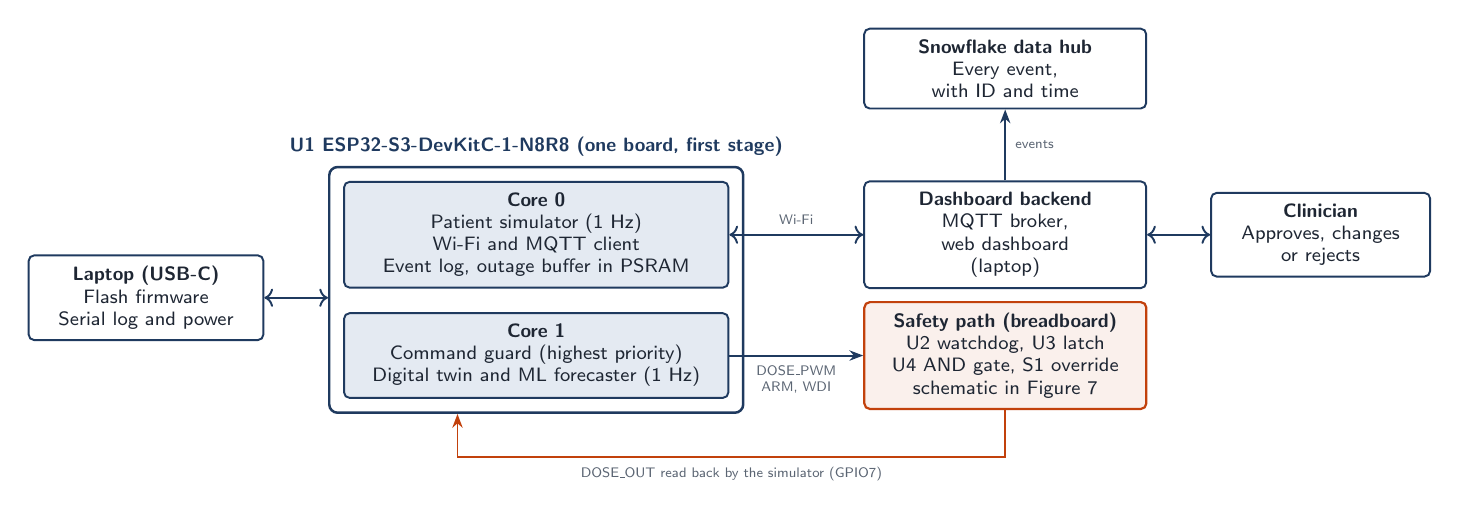
\begin{tikzpicture}[node distance=6mm]
\node[wbox, text width=27mm] (lap) {\textbf{Laptop (USB-C)}\\Flash firmware\\Serial log and power};
\node[box, text width=46mm, right=10mm of lap, yshift=8mm] (c0) {\textbf{Core 0}\\Patient simulator (1 Hz)\\Wi-Fi and MQTT client\\Event log, outage buffer in PSRAM};
\node[box, text width=46mm, below=3mm of c0] (c1) {\textbf{Core 1}\\Command guard (highest priority)\\Digital twin and ML forecaster (1 Hz)};
\begin{scope}[on background layer]
\node[draw=navy, fill=white, rounded corners=3pt, line width=0.9pt, fit=(c0)(c1), inner sep=5pt, label={[title]above:U1 ESP32-S3-DevKitC-1-N8R8 (one board, first stage)}] (u1) {};
\end{scope}
\node[hbox, text width=33mm, right=17mm of c1] (safe) {\textbf{Safety path (breadboard)}\\U2 watchdog, U3 latch\\U4 AND gate, S1 override\\schematic in Figure 7};
\node[wbox, text width=33mm, right=17mm of c0] (dash) {\textbf{Dashboard backend}\\MQTT broker, web dashboard\\(laptop)};
\node[wbox, text width=33mm, above=9mm of dash] (snow) {\textbf{Snowflake data hub}\\Every event, with ID and time};
\node[wbox, text width=25mm, right=8mm of dash] (clin) {\textbf{Clinician}\\Approves, changes\\or rejects};
\draw[arr, <->] (lap.east) -- (lap.east -| u1.west);
\draw[arr, <->] (c0.east) -- node[lab, above]{Wi-Fi} (dash.west);
\draw[arr] (dash) -- node[lab, right]{events} (snow);
\draw[arr, <->] (clin) -- (dash);
\draw[arr] (c1.east) -- node[lab, below, align=center]{DOSE\_PWM\\ARM, WDI} (safe.west);
\draw[arr, accent] (safe.south) -- ++(0,-6mm) -| node[lab, below, pos=0.25]{DOSE\_OUT read back by the simulator (GPIO7)} ($(u1.south)+(-10mm,0)$);
\end{tikzpicture}
\end{document}
